\documentclass[tikz]{standalone}
\usepackage{tikz}
\usepackage{../../../../glossary}
\usetikzlibrary{arrows.meta, chains, positioning}

\begin{document}

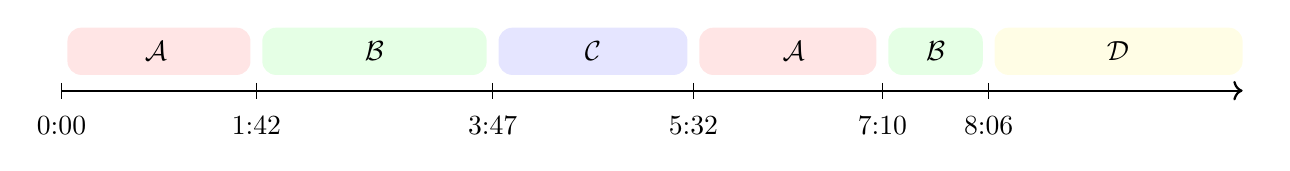
\begin{tikzpicture}[xscale=15] % Adjust xscale for A4 width

    % Draw the timeline
    \draw[->, thick] (0, 0) -- (1, 0) node[right] {};

    % \mathcal{A} section
    \fill[red!20, opacity=0.5, rounded corners=5] (0.005, 0.8) rectangle (0.16, 0.2);
    \fill[red!20, opacity=0.5, rounded corners=5] (0.54, 0.8) rectangle (0.69, 0.2);

    % \mathcal{B} section
    \fill[green!20, opacity=0.5, rounded corners=5] (0.17, 0.8) rectangle (0.36, 0.2);
    \fill[green!20, opacity=0.5, rounded corners=5] (0.7, 0.8) rectangle (0.78, 0.2);

    % \mathcal{C} section
    \fill[blue!20, opacity=0.5, rounded corners=5] (0.37, 0.8) rectangle (0.53, 0.2);

    % \mathcal{D} section
    \fill[yellow!20, opacity=0.5, rounded corners=5] (0.79, 0.8) rectangle (1, 0.2);
    
    % Add ticks and labels (example)
    \foreach \x/\label in {
            0.000/0:00, % A 
            0.165/1:42, % B
            0.365/3:47, % C
            0.535/5:32, % A
            0.695/7:10, % B
            0.785/8:06  % D
        } {
        \draw (\x, 0.1) -- (\x, -0.1); % Ticks
        \node[below] at (\x, -0.2) {\label}; % Labels
    }
    
    % Add example event descriptions aligned in the middle of the marks
    \foreach \x/\text in {
            0.08/$\mathcal{A}$, 
            0.265/$\mathcal{B}$, 
            0.45/$\mathcal{C}$, 
            0.62/$\mathcal{A}$, 
            0.74/$\mathcal{B}$,
            0.89442/$\mathcal{D}$
        } {
        \node[above, anchor=center] at (\x, 0.5) {\text};
    }
    
    \end{tikzpicture}
    

\end{document}